\chapter{Greedy algorithms}

\index{greedy algorithm}

A \key{greedy algorithm}
constructs a solution to the problem
by always making a choice that looks
the best at the moment.
A greedy algorithm never takes back
its choices, but directly constructs
the final solution.
For this reason, greedy algorithms
are usually very efficient.

The difficulty in designing greedy algorithms
is to find a greedy strategy
that always produces an optimal solution
to the problem.
The locally optimal choices in a greedy
algorithm should also be globally optimal.
It is often difficult to argue that
a greedy algorithm works.

\section{Coin problem}

As a first example, we consider a problem
where we are given a set of coins
and our task is to form a sum of money $n$
using the coins.
The values of the coins are
$\texttt{coins}=\{c_1,c_2,\ldots,c_k\}$,
and each coin can be used as many times we want.
What is the minimum number of coins needed?

For example, if the coins are the euro coins (in cents)
\[\{1,2,5,10,20,50,100,200\}\]
and $n=520$,
we need at least four coins.
The optimal solution is to select coins
$200+200+100+20$ whose sum is 520.

\subsubsection{Greedy algorithm}

A simple greedy algorithm to the problem
always selects the largest possible coin,
until the required sum of money has been constructed.
This algorithm works in the example case,
because we first select two 200 cent coins,
then one 100 cent coin and finally one 20 cent coin.
But does this algorithm always work?

It turns out that if the coins are the euro coins,
the greedy algorithm \emph{always} works, i.e.,
it always produces a solution with the fewest
possible number of coins.
The correctness of the algorithm can be
shown as follows:

First, each coin 1, 5, 10, 50 and 100 appears
at most once in an optimal solution,
because if the
solution would contain two such coins,
we could replace them by one coin and
obtain a better solution.
For example, if the solution would contain
coins $5+5$, we could replace them by coin $10$.

In the same way, coins 2 and 20 appear
at most twice in an optimal solution,
because we could replace
coins $2+2+2$ by coins $5+1$ and
coins $20+20+20$ by coins $50+10$.
Moreover, an optimal solution cannot contain
coins $2+2+1$ or $20+20+10$,
because we could replace them by coins $5$ and $50$.

Using these observations,
we can show for each coin $x$ that
it is not possible to optimally construct
a sum $x$ or any larger sum by only using coins
that are smaller than $x$.
For example, if $x=100$, the largest optimal
sum using the smaller coins is  $50+20+20+5+2+2=99$.
Thus, the greedy algorithm that always selects
the largest coin produces the optimal solution.

This example shows that it can be difficult
to argue that a greedy algorithm works,
even if the algorithm itself is simple.

\subsubsection{General case}

In the general case, the coin set can contain any coins
and the greedy algorithm \emph{does not} necessarily produce
an optimal solution.

We can prove that a greedy algorithm does not work
by showing a counterexample
where the algorithm gives a wrong answer.
In this problem we can easily find a counterexample:
if the coins are $\{1,3,4\}$ and the target sum
is 6, the greedy algorithm produces the solution
$4+1+1$ while the optimal solution is $3+3$.

It is not known if the general coin problem
can be solved using any greedy algorithm\footnote{However, it is possible
to \emph{check} in polynomial time
if the greedy algorithm presented in this chapter works for
a given set of coins \cite{pea05}.}.
However, as we will see in Chapter 7,
in some cases,
the general problem can be efficiently
solved using a dynamic
programming algorithm that always gives the
correct answer.

\section{Scheduling}

Many scheduling problems can be solved
using greedy algorithms.
A classic problem is as follows:
Given $n$ events with their starting and ending
times, find a schedule
that includes as many events as possible.
It is not possible to select an event partially.
For example, consider the following events:
\begin{center}
\begin{tabular}{lll}
event & starting time & ending time \\
\hline
$A$ & 1 & 3 \\
$B$ & 2 & 5 \\
$C$ & 3 & 9 \\
$D$ & 6 & 8 \\
\end{tabular}
\end{center}
In this case the maximum number of events is two.
For example, we can select events $B$ and $D$
as follows:
\begin{center}
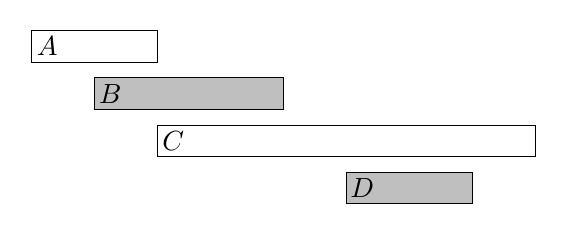
\begin{tikzpicture}[scale=.4]
  \begin{scope}
    \draw (2, 0) rectangle (6, -1);
    \draw[fill=lightgray] (4, -1.5) rectangle (10, -2.5);
    \draw (6, -3) rectangle (18, -4);
    \draw[fill=lightgray] (12, -4.5) rectangle (16, -5.5);
    \node at (2.5,-0.5) {$A$};
    \node at (4.5,-2) {$B$};
    \node at (6.5,-3.5) {$C$};
    \node at (12.5,-5) {$D$};
  \end{scope}
\end{tikzpicture}
\end{center}

It is possible to invent several greedy algorithms
for the problem, but which of them works in every case?

\subsubsection*{Algorithm 1}

The first idea is to select as \emph{short}
events as possible.
In the example case this algorithm
selects the following events:
\begin{center}
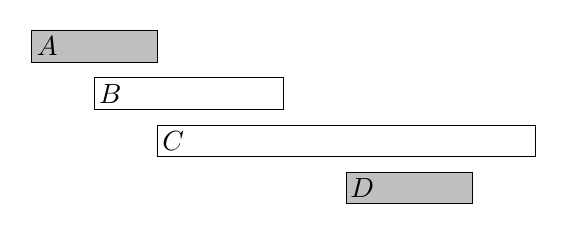
\begin{tikzpicture}[scale=.4]
  \begin{scope}
    \draw[fill=lightgray] (2, 0) rectangle (6, -1);
    \draw (4, -1.5) rectangle (10, -2.5);
    \draw (6, -3) rectangle (18, -4);
    \draw[fill=lightgray] (12, -4.5) rectangle (16, -5.5);
    \node at (2.5,-0.5) {$A$};
    \node at (4.5,-2) {$B$};
    \node at (6.5,-3.5) {$C$};
    \node at (12.5,-5) {$D$};
  \end{scope}
\end{tikzpicture}
\end{center}

However, selecting short events is not always
a correct strategy. For example, the algorithm fails
in the following case:
\begin{center}
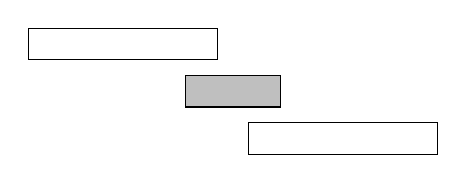
\begin{tikzpicture}[scale=.4]
  \begin{scope}
    \draw (1, 0) rectangle (7, -1);
    \draw[fill=lightgray] (6, -1.5) rectangle (9, -2.5);
    \draw (8, -3) rectangle (14, -4);
  \end{scope}
\end{tikzpicture}
\end{center}
If we select the short event, we can only select one event.
However, it would be possible to select both long events.

\subsubsection*{Algorithm 2}

Another idea is to always select the next possible
event that \emph{begins} as \emph{early} as possible.
This algorithm selects the following events:
\begin{center}
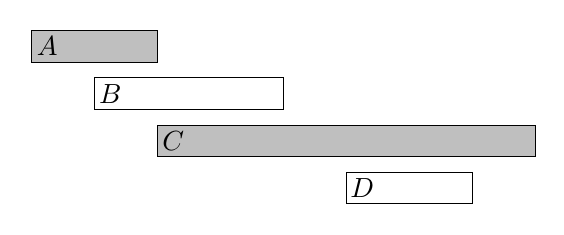
\begin{tikzpicture}[scale=.4]
  \begin{scope}
    \draw[fill=lightgray] (2, 0) rectangle (6, -1);
    \draw (4, -1.5) rectangle (10, -2.5);
    \draw[fill=lightgray] (6, -3) rectangle (18, -4);
    \draw (12, -4.5) rectangle (16, -5.5);
    \node at (2.5,-0.5) {$A$};
    \node at (4.5,-2) {$B$};
    \node at (6.5,-3.5) {$C$};
    \node at (12.5,-5) {$D$};
  \end{scope}
\end{tikzpicture}
\end{center}

However, we can find a counterexample
also for this algorithm.
For example, in the following case,
the algorithm only selects one event:
\begin{center}
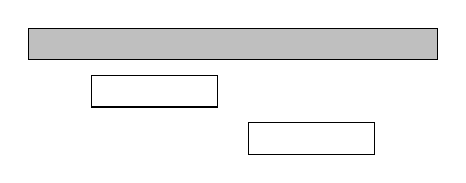
\begin{tikzpicture}[scale=.4]
  \begin{scope}
    \draw[fill=lightgray] (1, 0) rectangle (14, -1);
    \draw (3, -1.5) rectangle (7, -2.5);
    \draw (8, -3) rectangle (12, -4);
  \end{scope}
\end{tikzpicture}
\end{center}
If we select the first event, it is not possible
to select any other events.
However, it would be possible to select the
other two events.

\subsubsection*{Algorithm 3}

The third idea is to always select the next
possible event that \emph{ends} as \emph{early} as possible.
This algorithm selects the following events: 
\begin{center}
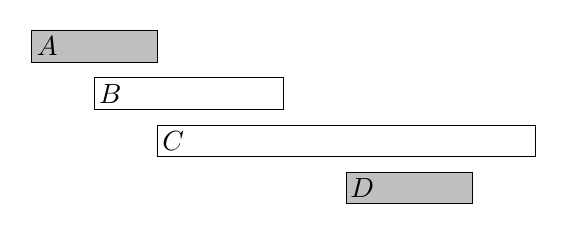
\begin{tikzpicture}[scale=.4]
  \begin{scope}
    \draw[fill=lightgray] (2, 0) rectangle (6, -1);
    \draw (4, -1.5) rectangle (10, -2.5);
    \draw (6, -3) rectangle (18, -4);
    \draw[fill=lightgray] (12, -4.5) rectangle (16, -5.5);
    \node at (2.5,-0.5) {$A$};
    \node at (4.5,-2) {$B$};
    \node at (6.5,-3.5) {$C$};
    \node at (12.5,-5) {$D$};
  \end{scope}
\end{tikzpicture}
\end{center}

It turns out that this algorithm
\emph{always} produces an optimal solution.
The reason for this is that it is always an optimal choice
to first select an event that ends
as early as possible.
After this, it is an optimal choice
to select the next event
using the same strategy, etc.,
until we cannot select any more events.

One way to argue that the algorithm works
is to consider
what happens if we first select an event
that ends later than the event that ends
as early as possible.
Now, we will have at most an equal number of
choices how we can select the next event.
Hence, selecting an event that ends later
can never yield a better solution,
and the greedy algorithm is correct.

\section{Tasks and deadlines}

Let us now consider a problem where
we are given $n$ tasks with durations and deadlines
and our task is to choose an order to perform the tasks.
For each task, we earn $d-x$ points
where $d$ is the task's deadline
and $x$ is the moment when we finish the task.
What is the largest possible total score
we can obtain?

For example, suppose that the tasks are as follows:
\begin{center}
\begin{tabular}{lll}
task & duration & deadline \\
\hline
$A$ & 4 & 2 \\
$B$ & 3 & 5 \\
$C$ & 2 & 7 \\
$D$ & 4 & 5 \\
\end{tabular}
\end{center}
In this case, an optimal schedule for the tasks
is as follows:
\begin{center}
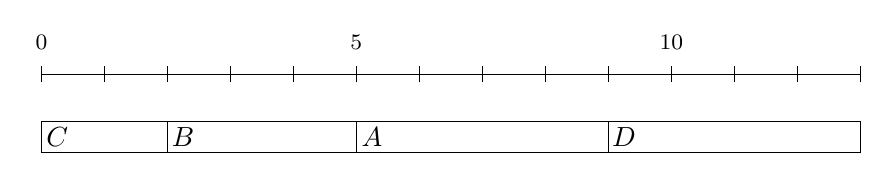
\begin{tikzpicture}[scale=.4]
  \begin{scope}
    \draw (0, 0) rectangle (4, -1);
    \draw (4, 0) rectangle (10, -1);
    \draw (10, 0) rectangle (18, -1);
    \draw (18, 0) rectangle (26, -1);
    \node at (0.5,-0.5) {$C$};
    \node at (4.5,-0.5) {$B$};
    \node at (10.5,-0.5) {$A$};
    \node at (18.5,-0.5) {$D$};

    \draw (0,1.5) -- (26,1.5);
    \foreach \i in {0,2,...,26}
    {
        \draw (\i,1.25) -- (\i,1.75);
    }
    \footnotesize
    \node at (0,2.5) {0};
    \node at (10,2.5) {5};
    \node at (20,2.5) {10};

  \end{scope}
\end{tikzpicture}
\end{center}
In this solution, $C$ yields 5 points,
$B$ yields 0 points, $A$ yields $-7$ points
and $D$ yields $-8$ points,
so the total score is $-10$.

Surprisingly, the optimal solution to the problem
does not depend on the deadlines at all,
but a correct greedy strategy is to simply
perform the tasks \emph{sorted by their durations}
in increasing order.
The reason for this is that if we ever perform
two tasks one after another such that the first task
takes longer than the second task,
we can obtain a better solution if we swap the tasks.
For example, consider the following schedule:
\begin{center}
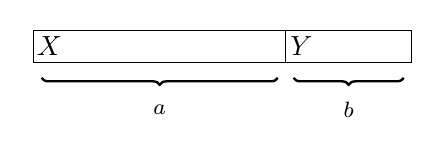
\begin{tikzpicture}[scale=.4]
  \begin{scope}
    \draw (0, 0) rectangle (8, -1);
    \draw (8, 0) rectangle (12, -1);
    \node at (0.5,-0.5) {$X$};
    \node at (8.5,-0.5) {$Y$};

\draw [decoration={brace}, decorate, line width=0.3mm] (7.75,-1.5) -- (0.25,-1.5);
\draw [decoration={brace}, decorate, line width=0.3mm] (11.75,-1.5) -- (8.25,-1.5);

\footnotesize
\node at (4,-2.5) {$a$};
\node at (10,-2.5) {$b$};

  \end{scope}
\end{tikzpicture}
\end{center}
Here $a>b$, so we should swap the tasks:
\begin{center}
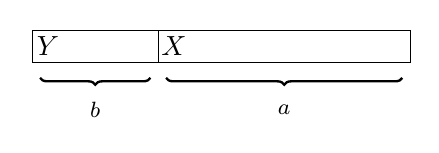
\begin{tikzpicture}[scale=.4]
  \begin{scope}
    \draw (0, 0) rectangle (4, -1);
    \draw (4, 0) rectangle (12, -1);
    \node at (0.5,-0.5) {$Y$};
    \node at (4.5,-0.5) {$X$};

\draw [decoration={brace}, decorate, line width=0.3mm] (3.75,-1.5) -- (0.25,-1.5);
\draw [decoration={brace}, decorate, line width=0.3mm] (11.75,-1.5) -- (4.25,-1.5);

\footnotesize
\node at (2,-2.5) {$b$};
\node at (8,-2.5) {$a$};

  \end{scope}
\end{tikzpicture}
\end{center}
Now $X$ gives $b$ points less and $Y$ gives $a$ points more,
so the total score increases by $a-b > 0$.
In an optimal solution,
for any two consecutive tasks,
it must hold that the shorter task comes
before the longer task.
Thus, the tasks must be performed
sorted by their durations.

\section{Minimizing sums}

We next consider a problem where
we are given $n$ numbers $a_1,a_2,\ldots,a_n$
and our task is to find a value $x$
that minimizes the sum
\[|a_1-x|^c+|a_2-x|^c+\cdots+|a_n-x|^c.\]
We focus on the cases $c=1$ and $c=2$.

\subsubsection{Case $c=1$}

In this case, we should minimize the sum
\[|a_1-x|+|a_2-x|+\cdots+|a_n-x|.\]
For example, if the numbers are $[1,2,9,2,6]$,
the best solution is to select $x=2$
which produces the sum
\[
|1-2|+|2-2|+|9-2|+|2-2|+|6-2|=12.
\]
In the general case, the best choice for $x$
is the \textit{median} of the numbers,
i.e., the middle number after sorting.
For example, the list $[1,2,9,2,6]$
becomes $[1,2,2,6,9]$ after sorting,
so the median is 2.

The median is an optimal choice,
because if $x$ is smaller than the median,
the sum becomes smaller by increasing $x$,
and if $x$ is larger then the median,
the sum becomes smaller by decreasing $x$.
Hence, the optimal solution is that $x$
is the median.
If $n$ is even and there are two medians,
both medians and all values between them
are optimal choices.

\subsubsection{Case $c=2$}

In this case, we should minimize the sum
\[(a_1-x)^2+(a_2-x)^2+\cdots+(a_n-x)^2.\]
For example, if the numbers are $[1,2,9,2,6]$,
the best solution is to select $x=4$
which produces the sum
\[
(1-4)^2+(2-4)^2+(9-4)^2+(2-4)^2+(6-4)^2=46.
\]
In the general case, the best choice for $x$
is the \emph{average} of the numbers.
In the example the average is $(1+2+9+2+6)/5=4$.
This result can be derived by presenting
the sum as follows:
\[
nx^2 - 2x(a_1+a_2+\cdots+a_n) + (a_1^2+a_2^2+\cdots+a_n^2)
\]
The last part does not depend on $x$,
so we can ignore it.
The remaining parts form a function
$nx^2-2xs$ where $s=a_1+a_2+\cdots+a_n$.
This is a parabola opening upwards
with roots $x=0$ and $x=2s/n$,
and the minimum value is the average
of the roots $x=s/n$, i.e.,
the average of the numbers $a_1,a_2,\ldots,a_n$.

\section{Data compression}

\index{data compression}
\index{binary code}
\index{codeword}

A \key{binary code} assigns for each character
of a string a \key{codeword} that consists of bits.
We can \emph{compress} the string using the binary code
by replacing each character by the
corresponding codeword.
For example, the following binary code
assigns codewords for characters
\texttt{A}–\texttt{D}:
\begin{center}
\begin{tabular}{rr}
character & codeword \\
\hline
\texttt{A} & 00 \\
\texttt{B} & 01 \\
\texttt{C} & 10 \\
\texttt{D} & 11 \\
\end{tabular}
\end{center}
This is a \key{constant-length} code
which means that the length of each
codeword is the same.
For example, we can compress the string
\texttt{AABACDACA} as follows:
\[00\,00\,01\,00\,10\,11\,00\,10\,00\]
Using this code, the length of the compressed
string is 18 bits.
However, we can compress the string better
if we use a \key{variable-length} code
where codewords may have different lengths.
Then we can give short codewords for
characters that appear often
and long codewords for characters
that appear rarely.
It turns out that an \key{optimal} code
for the above string is as follows:
\begin{center}
\begin{tabular}{rr}
character & codeword \\
\hline
\texttt{A} & 0 \\
\texttt{B} & 110 \\
\texttt{C} & 10 \\
\texttt{D} & 111 \\
\end{tabular}
\end{center}
An optimal code produces a compressed string
that is as short as possible.
In this case, the compressed string using
the optimal code is
\[0\,0\,110\,0\,10\,111\,0\,10\,0,\]
so only 15 bits are needed instead of 18 bits.
Thus, thanks to a better code it was possible to
save 3 bits in the compressed string.

We require that no codeword
is a prefix of another codeword.
For example, it is not allowed that a code
would contain both codewords 10
and 1011.
The reason for this is that we want
to be able to generate the original string
from the compressed string.
If a codeword could be a prefix of another codeword,
this would not always be possible.
For example, the following code is \emph{not} valid:
\begin{center}
\begin{tabular}{rr}
character & codeword \\
\hline
\texttt{A} & 10 \\
\texttt{B} & 11 \\
\texttt{C} & 1011 \\
\texttt{D} & 111 \\
\end{tabular}
\end{center}
Using this code, it would not be possible to know
if the compressed string 1011 corresponds to
the string \texttt{AB} or the string \texttt{C}.

\index{Huffman coding}

\subsubsection{Huffman coding}

\key{Huffman coding}\footnote{D. A. Huffman discovered this method
when solving a university course assignment
and published the algorithm in 1952 \cite{huf52}.} is a greedy algorithm
that constructs an optimal code for
compressing a given string.
The algorithm builds a binary tree
based on the frequencies of the characters
in the string,
and each character's codeword can be read
by following a path from the root to
the corresponding node.
A move to the left corresponds to bit 0,
and a move to the right corresponds to bit 1.

Initially, each character of the string is
represented by a node whose weight is the
number of times the character occurs in the string.
Then at each step two nodes with minimum weights
are combined by creating
a new node whose weight is the sum of the weights
of the original nodes.
The process continues until all nodes have been combined.

Next we will see how Huffman coding creates
the optimal code for the string
\texttt{AABACDACA}.
Initially, there are four nodes that correspond
to the characters of the string:

\begin{center}
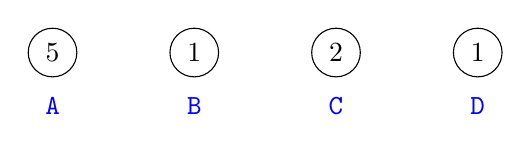
\begin{tikzpicture}[scale=0.9]
\node[draw, circle] (1) at (0,0) {$5$};
\node[draw, circle] (2) at (2,0) {$1$};
\node[draw, circle] (3) at (4,0) {$2$};
\node[draw, circle] (4) at (6,0) {$1$};

\node[color=blue] at (0,-0.75) {\texttt{A}};
\node[color=blue] at (2,-0.75) {\texttt{B}};
\node[color=blue] at (4,-0.75) {\texttt{C}};
\node[color=blue] at (6,-0.75) {\texttt{D}};

%\path[draw,thick,-] (4) -- (5);
\end{tikzpicture}
\end{center}
The node that represents character \texttt{A}
has weight 5 because character \texttt{A}
appears 5 times in the string.
The other weights have been calculated
in the same way.

The first step is to combine the nodes that
correspond to characters \texttt{B} and \texttt{D},
both with weight 1.
The result is:
\begin{center}
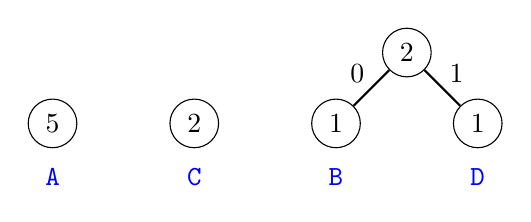
\begin{tikzpicture}[scale=0.9]
\node[draw, circle] (1) at (0,0) {$5$};
\node[draw, circle] (3) at (2,0) {$2$};
\node[draw, circle] (2) at (4,0) {$1$};
\node[draw, circle] (4) at (6,0) {$1$};
\node[draw, circle] (5) at (5,1) {$2$};

\node[color=blue] at (0,-0.75) {\texttt{A}};
\node[color=blue] at (2,-0.75) {\texttt{C}};
\node[color=blue] at (4,-0.75) {\texttt{B}};
\node[color=blue] at (6,-0.75) {\texttt{D}};

\node at (4.3,0.7) {0};
\node at (5.7,0.7) {1};

\path[draw,thick,-] (2) -- (5);
\path[draw,thick,-] (4) -- (5);
\end{tikzpicture}
\end{center}
After this, the nodes with weight 2 are combined:
\begin{center}
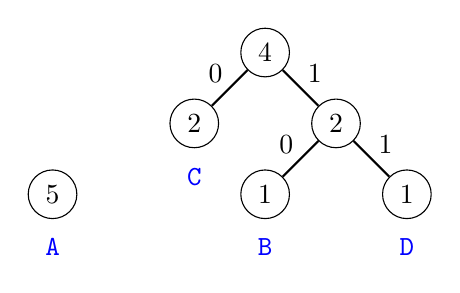
\begin{tikzpicture}[scale=0.9]
\node[draw, circle] (1) at (1,0) {$5$};
\node[draw, circle] (3) at (3,1) {$2$};
\node[draw, circle] (2) at (4,0) {$1$};
\node[draw, circle] (4) at (6,0) {$1$};
\node[draw, circle] (5) at (5,1) {$2$};
\node[draw, circle] (6) at (4,2) {$4$};

\node[color=blue] at (1,-0.75) {\texttt{A}};
\node[color=blue] at (3,1-0.75) {\texttt{C}};
\node[color=blue] at (4,-0.75) {\texttt{B}};
\node[color=blue] at (6,-0.75) {\texttt{D}};

\node at (4.3,0.7) {0};
\node at (5.7,0.7) {1};
\node at (3.3,1.7) {0};
\node at (4.7,1.7) {1};

\path[draw,thick,-] (2) -- (5);
\path[draw,thick,-] (4) -- (5);
\path[draw,thick,-] (3) -- (6);
\path[draw,thick,-] (5) -- (6);
\end{tikzpicture}
\end{center}
Finally, the two remaining nodes are combined:
\begin{center}
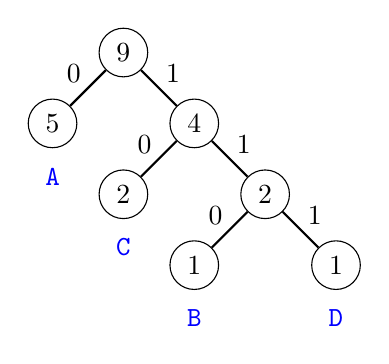
\begin{tikzpicture}[scale=0.9]
\node[draw, circle] (1) at (2,2) {$5$};
\node[draw, circle] (3) at (3,1) {$2$};
\node[draw, circle] (2) at (4,0) {$1$};
\node[draw, circle] (4) at (6,0) {$1$};
\node[draw, circle] (5) at (5,1) {$2$};
\node[draw, circle] (6) at (4,2) {$4$};
\node[draw, circle] (7) at (3,3) {$9$};

\node[color=blue] at (2,2-0.75) {\texttt{A}};
\node[color=blue] at (3,1-0.75) {\texttt{C}};
\node[color=blue] at (4,-0.75) {\texttt{B}};
\node[color=blue] at (6,-0.75) {\texttt{D}};

\node at (4.3,0.7) {0};
\node at (5.7,0.7) {1};
\node at (3.3,1.7) {0};
\node at (4.7,1.7) {1};
\node at (2.3,2.7) {0};
\node at (3.7,2.7) {1};

\path[draw,thick,-] (2) -- (5);
\path[draw,thick,-] (4) -- (5);
\path[draw,thick,-] (3) -- (6);
\path[draw,thick,-] (5) -- (6);
\path[draw,thick,-] (1) -- (7);
\path[draw,thick,-] (6) -- (7);
\end{tikzpicture}
\end{center}

Now all nodes are in the tree, so the code is ready.
The following codewords can be read from the tree:
\begin{center}
\begin{tabular}{rr}
character & codeword \\
\hline
\texttt{A} & 0 \\
\texttt{B} & 110 \\
\texttt{C} & 10 \\
\texttt{D} & 111 \\
\end{tabular}
\end{center}
